\section{Current Infrastructure}

In this section we will describe the current computing infrastructure
maintained by the Configuration Team.

\subsection{Puppet Masters}

% UPDATE numbers and split batch from interactive

\begin{figure}[H]
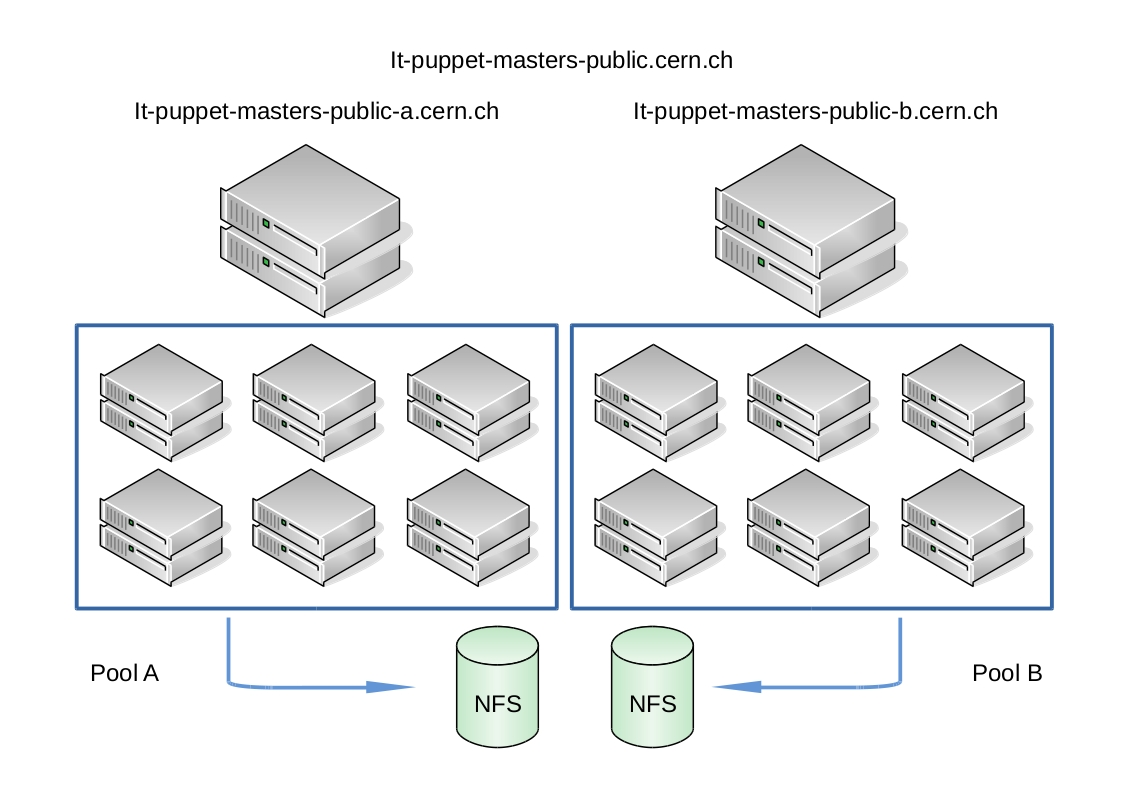
\includegraphics[width=\textwidth,height=\textheight,keepaspectratio]{ConfigurationManagement/Infrastructure_pm.jpg}
\caption{Puppet masters infrastructure}
\end{figure}

The image outlines the current puppet master infrastructure. As we can see
there are two different clusters (also called pools) taking care of
compiling puppet manifests. Every pool has two load balancers spreading
the load equally between all the servers in the pool: the requests are
always forwarded to the less loaded server of the pool. Every pool has
approximately 40 machines with four cores and eight GigaBytes of memory.

Each pool is split in two clusters: the interactive cluster and the batch
cluster. The interactive cluster is smaller (usually around three
machines) and takes care of all the Puppet runs triggered using the
command line; most of the testing runs are compiled with this one. The
batch cluster instead compiles all the runs that are triggered in the
background by the puppet daemon. When a machine is spawned using OpenStack
it is assigned randomly to one of the two pools and stays there for the
whole lifecycle.

The servers read the puppet code from two different NFS shares, one for
each pool. The NFS share is populated by Jens as we will see it in the
next sections. This helps to balance the load across two different pools,
avoiding to overload one of them. In case of failures of one pool, the
machines can fallback on the healthy one in case of emergency. 

\subsection{Foreman}

Foreman manages the lifecycle of the machines, giving to the service
managers an overview of their servers using a web interface. It contains
the correspondences between a server and its hostgroup/environment, it
allows to browse Puppet reports and also manage physical machines.

As we can see from the image Foreman is split in four different services,
all using the same database instance; all the traffic is redirected to the
correct service using load balancers. Depending on the port, the balancers
redirect the traffic to the correct servers.

\begin{figure}[H]
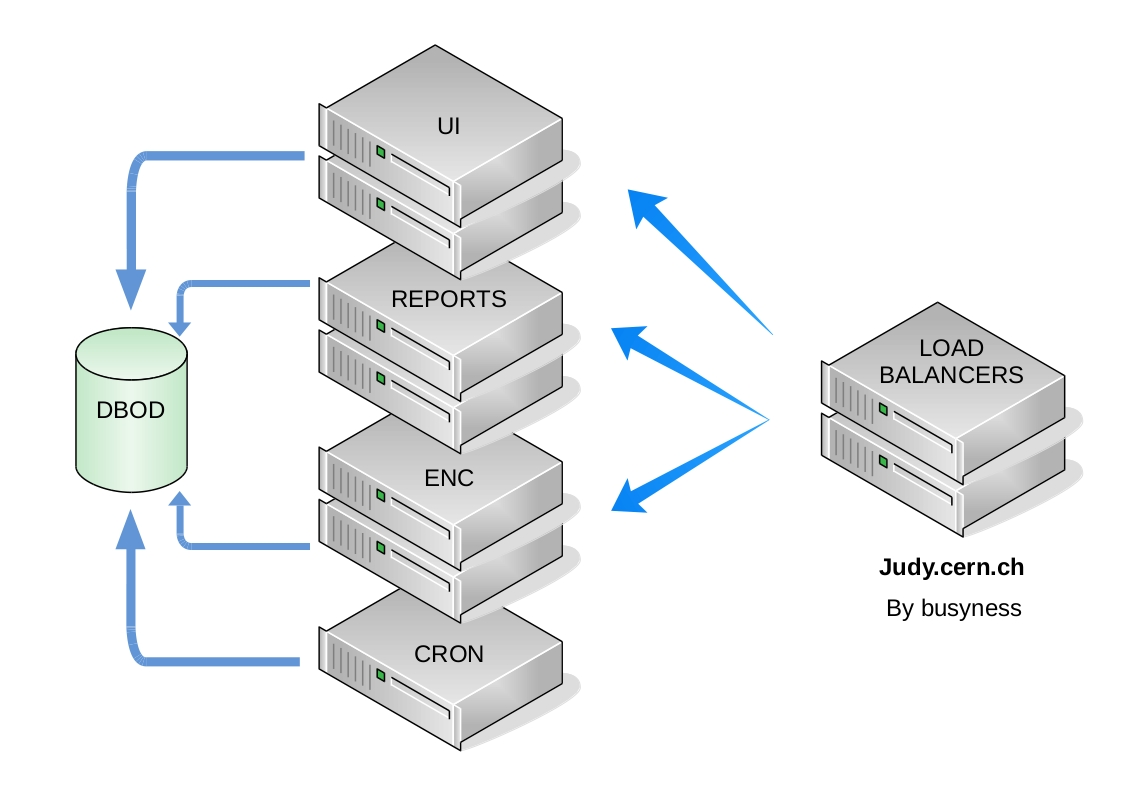
\includegraphics[width=\textwidth,height=\textheight,keepaspectratio]{ConfigurationManagement/Infrastructure_judy.jpg}
\caption{Foreman Infrastructure}
\end{figure}

The ENC service of Foreman gives to the Puppet masters the correspondence
between a machine name and the hostgroup/environment it is assigned to.

% TODO expand a bit

\subsection{Jens and PuppetDb}

\begin{figure}[H]
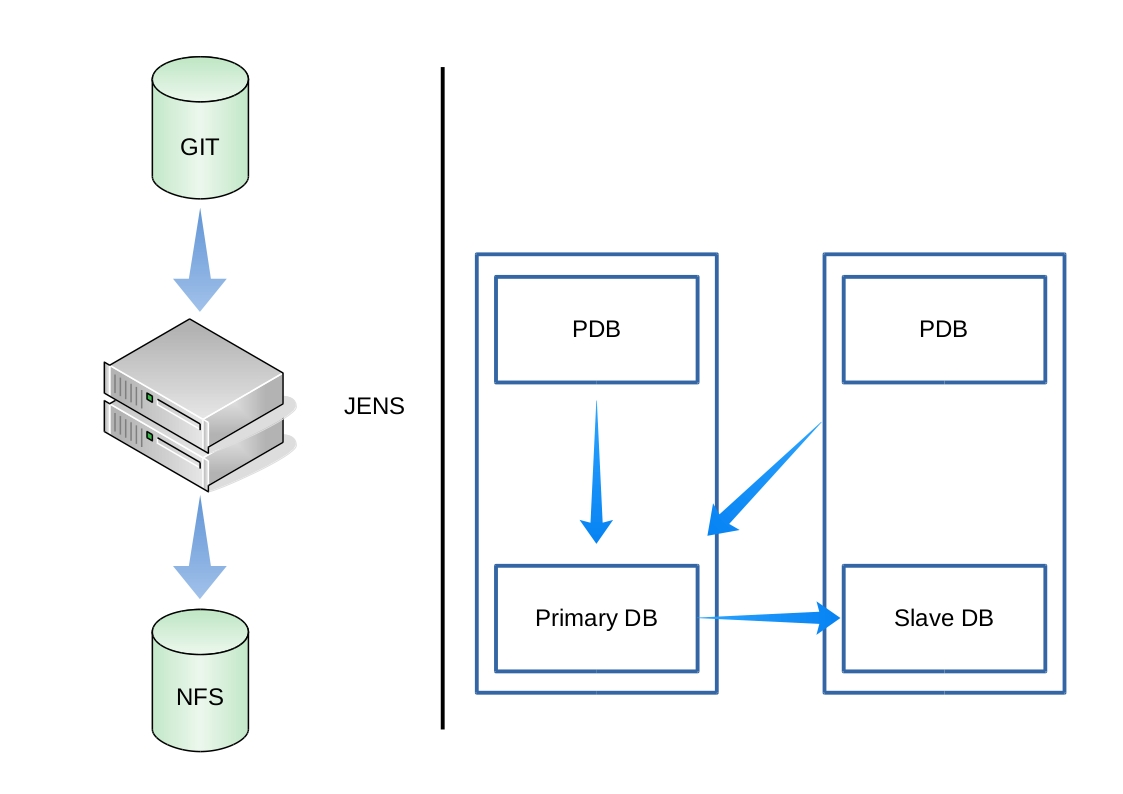
\includegraphics[width=\textwidth,height=\textheight,keepaspectratio]{ConfigurationManagement/Infrastructure_jens_pdb.jpg}
\caption{Jens and PuppetDb infrastructure}
\end{figure}

The image above describes the current configuration of PuppetDb and Jens.
Starting from the left, we can see that Jens periodically polls the Git
repositories to get the changes in the modules, hostgroups and
environments.

Jens consequentially populates the Puppet tree accordingly to the
configuration specified in those files and shares it on a network mounted
NFS volume. Every Puppet pool mounts an NFS share, so there are two
different shares, one per pool, and two different Jens instances
populating the Puppet tree. All the Puppet master read the configuration
from the NFS volume of their pool and compile the catalogs accordingly.

PuppetDb stores all the Puppet reports and facts from the hosts and makes
them available in a database-like fashion. The result is an inventory of
metadata about every host in the infrastructure; this inventory is
queryable by users and by Puppet itself to retrieve information at
compilation time.
